\section{Method}

\begin{figure*}[t]
\begin{center}
% 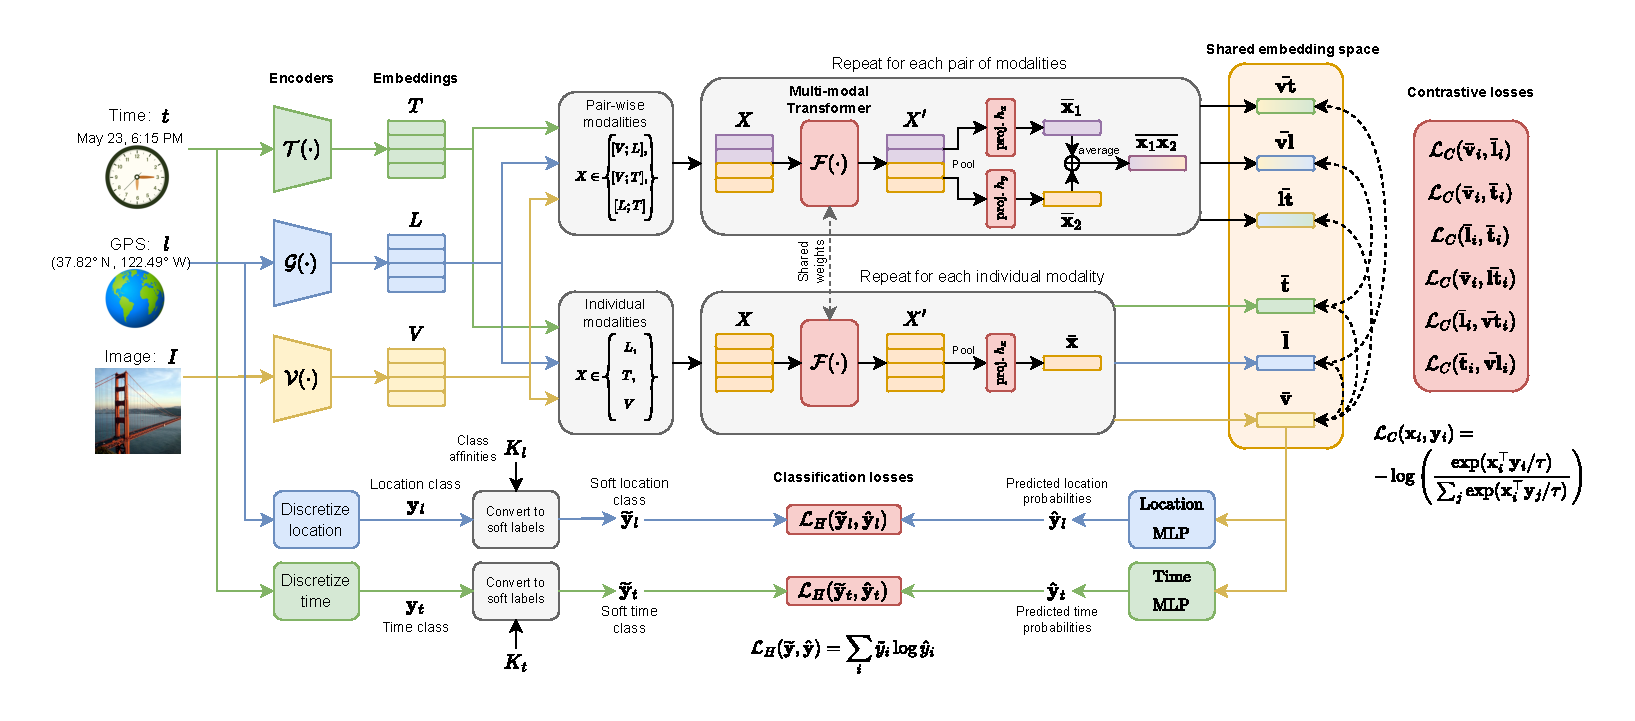
\includegraphics[width=0.95\linewidth]{figures/architecture_v2.pdf}
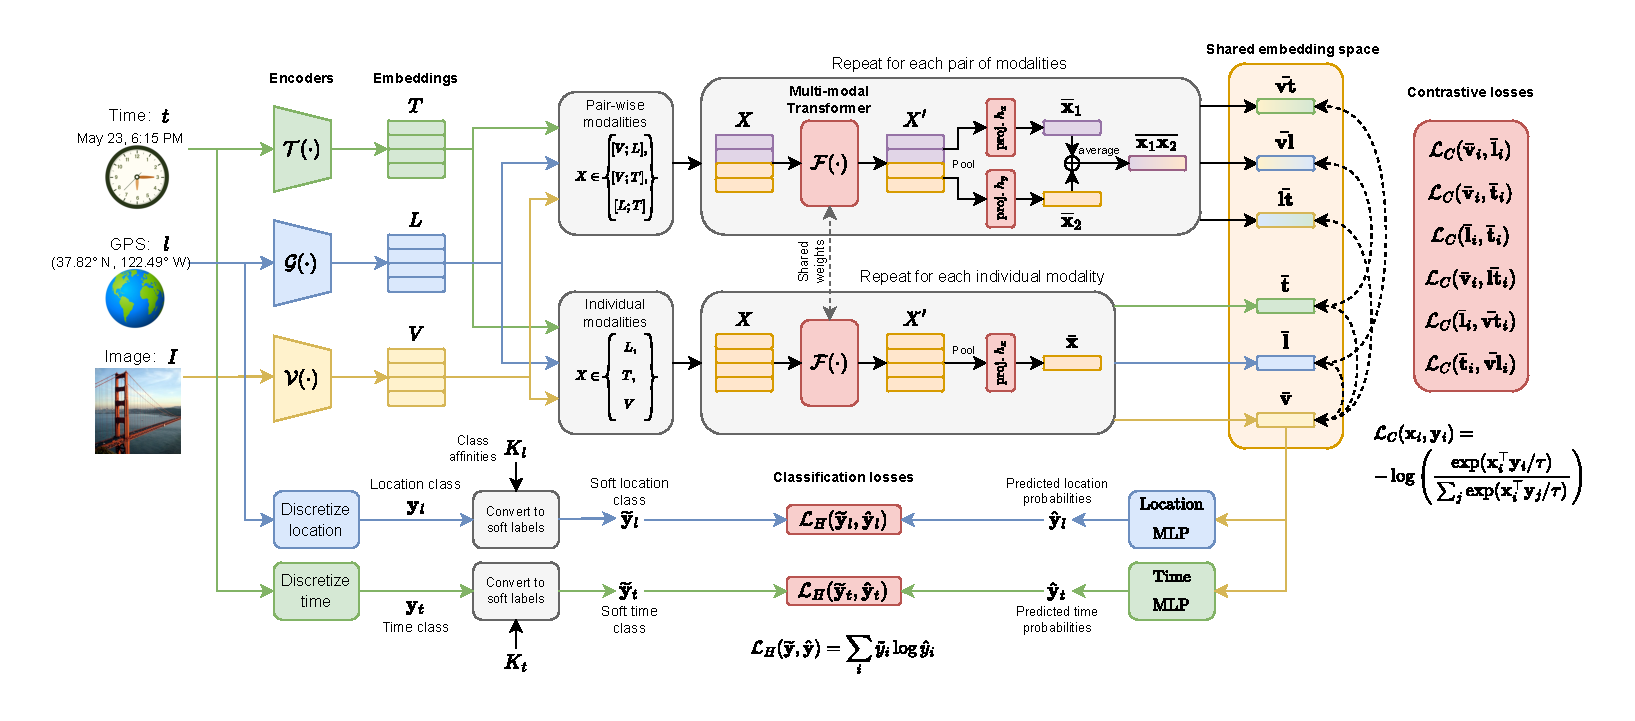
\includegraphics[
    width=0.925\linewidth,
    trim=0.75cm 0.5cm 0.75cm 0.5cm,
    clip
]{figures/architecture_v2.pdf}
\end{center}
\vspace{-2em}
\caption{\textbf{Architecture of \tiger.} Given an image $I$, GPS coordinates $l$, and timestamp $t$, modality-specific encoders produce visual ($V$), location ($L$), and temporal ($T$) embeddings. 
    Individual and pair-wise modality tokens are passed through a \textit{shared multi-modal transformer} $\mathcal{F}(\cdot)$, which employs self-attention to learn geo-temporal interactions. 
    Pooled embeddings are projected into a \textit{shared embedding space}, where a \textbf{contrastive loss} aligns unimodal and fused representations across all modality pairings (e.g., $V$--$L$, $V$--$T$, $L$--$T$). In parallel, the \textbf{classification losses with metric targets} on discretized location and time classes encourage the model to learn hierarchical cross-modal representations that vary smoothly across the embedding space.
\
}
\label{fig:architecture}
\end{figure*}


Our goal is to learn a unified representation that jointly embeds the location, visual, and time modalities, namely, the image $I$, GPS coordinates $l$, and time $t$ into a shared geo-temporal feature space. The representation is designed to preserve location identity while capturing temporal variation, enabling flexible cross-modal retrieval. Our proposed model is capable of  various tasks, such as, (i) retrieve an image of the same place at a different time, (ii) estimate the geo-location from image alone, and (iii) predict a plausible time-of-capture from single image or (iv) combined image and location cues. 

\subsection{Problem Statement}

Given a dataset $S_{\mathrm{train}}=\{(I_i, l_i, t_i)\}_{i=1}^N$, where $I_i$ is an image, $l_i$ denotes its GPS coordinates, and $t_i$ its capture time, our goal is to learn a model $f:\mathcal{M}\!\rightarrow\!\mathbb{R}^d$ that maps an input $\mathcal{M}$ from the modality set $\{I, l, t, (I,l), (I,t), (l,t)\}$ into a shared feature space $\mathbb{R}^d$. The model is trained so that features from inputs describing similar geo-temporal conditions (\textit{i.e.}, captured at nearby locations and times) have high cosine similarity, while unrelated inputs are pushed apart.

\subsection{Architecture}

Our model comprises three stages (see  Figure \ref{fig:architecture}). The first stage includes an image encoder $\mathcal{V}(I)=V\!\in\!\mathbb{R}^{N_V\times d}$, a location encoder $\mathcal{G}(l)=L\!\in\!\mathbb{R}^{N_L\times d}$, and a time encoder $\mathcal{T}(t)=T\!\in\!\mathbb{R}^{N_T\times d}$, where $N_V$, $N_L$, and $N_T$ denote the number of tokens per modality and $d$ the embedding dimension. The image encoder is a frozen CLIP ViT \cite{clip} that outputs one \texttt{[CLS]} token and $N_V\!-\!1$ patch embeddings. The location and time encoders use random Fourier features (RFF) to project 2D inputs into $N_L$ and $N_T$ high-dimensional vectors, modulated by frequencies $\sigma_i\!\in\!\{2^{2i}\}_{i=0}^{N-1}$. Each modality embedding is then linearly projected and layer-normalized.

The second stage employs a multi-modal transformer $\mathcal{F}$ to refine the modality-specific embeddings, learning fine-grained relationships between them via self-attention. Since there are six possible input combinations, $\{V,L,T,[V;L], [V;T], [L;T]\}$, we perform six forward passes during training. When two modalities are provided, we concatenate their embeddings along the token dimension before fusion, i.e., $X\!\in\!\{V,L,T,[V;L],[V;T],[L;T]\}$ and obtain $X'=\mathcal{F}(X)$.

For each refined embedding $X'$, we perform pooling to aggregate token representations and then project them into the shared embedding space via learned projections $h_x(\cdot)$:
\[
\mathbf{x}=\tfrac{1}{N_x}\sum_{i=1}^{N_x}X'_{i,:},\quad 
\mathbf{x}'=h_x(\mathbf{x}),\quad 
f(x)=\bar{\mathbf{x}}=\tfrac{\mathbf{x}'}{\|\mathbf{x}'\|},
\]
Similarly for bimodal inputs, we first pool and project each constituent modality to obtain embeddings $\bar{\mathbf{x}}_1$ and $\bar{\mathbf{x}}_2$, 
following the same procedure used for unimodal inputs. The resulting normalized embeddings are then fused by averaging: 
\[
f(x_1, x_2) = 
\frac{\bar{\mathbf{x}}_1 + \bar{\mathbf{x}}_2}{
\|\bar{\mathbf{x}}_1 + \bar{\mathbf{x}}_2\|}.
\]
This yields six embeddings $\{\bar{\mathbf{v}}, \bar{\mathbf{l}}, \bar{\mathbf{t}}, \bar{\mathbf{vl}}, \bar{\mathbf{vt}}, \bar{\mathbf{lt}}\}$, all residing in a shared geo-temporal feature space.

\subsection{Losses}

\tiger is optimized using a combination of contrastive and classification losses with soft metric targets. The contrastive objectives encourage embeddings from different input modalities to align within the shared feature space, forming the foundation for all geo-temporal retrieval tasks. In parallel, a classification loss is applied only to the final image embeddings $\bar{\mathbf{v}}$, enforcing a smooth, structured organization of the embedding space guided by the soft metric targets.

\noindent\textbf{Contrastive losses.}
We employ five contrastive objectives to align all meaningful modality pairs, excluding the individual location and time embeddings $(\bar{\mathbf{l}},\bar{\mathbf{t}})$, which remain uncorrelated. Specifically, we optimize the pairs $(\bar{\mathbf{v}},\bar{\mathbf{l}})$, $(\bar{\mathbf{v}},\bar{\mathbf{t}})$, $(\bar{\mathbf{v}},\bar{\mathbf{lt}})$, $(\bar{\mathbf{l}},\bar{\mathbf{vt}})$, and $(\bar{\mathbf{t}},\bar{\mathbf{vl}})$. Each pair $(\mathbf{x}_i,\mathbf{y}_i)$ is trained using the InfoNCE loss~\cite{oord2018representation}:

\begin{equation}
\mathcal{L}_C^{(i)}(\mathbf{x}_i,\mathbf{y}_i)
= -\log \frac{\exp(\mathbf{x}_i^\top \mathbf{y}_i / \tau)}{\sum_j \exp(\mathbf{x}_i^\top \mathbf{y}_j / \tau)},
\end{equation}
where $\tau$ is a temperature parameter controlling the sharpness of the distribution. The overall contrastive objective is the sum of all pairwise components:
\begin{equation}
\begin{aligned}
\mathcal{L}_C
= &\; \mathcal{L}_C(\bar{\mathbf{v}},\bar{\mathbf{l}})
+ \mathcal{L}_C(\bar{\mathbf{v}},\bar{\mathbf{t}})
+ \mathcal{L}_C(\bar{\mathbf{v}},\bar{\mathbf{lt}}) \\
&+ \mathcal{L}_C(\bar{\mathbf{l}},\bar{\mathbf{vt}})
+ \mathcal{L}_C(\bar{\mathbf{t}},\bar{\mathbf{vl}}).
\end{aligned}
\label{eq:contrastive-losses}
\end{equation}

\noindent\textbf{Classification losses.}
To encourage the model to learn geo-temporal representations that vary smoothly across the embedding space, we employ two classification losses with soft targets on the image embedding $\bar{\mathbf{v}}$.

\textit{Geo-location classes.}  
We define spatial classes using the Hierarchical Equal Area isoLatitude Pixelisation (HEALPix) \cite{gorski2005healpix} scheme, which divides the Earth's surface into equal-area regions whose centers lie on discretized latitude circles. The base resolution yields 12 cells, and each subdivision increases the count fourfold. We use the fourth hierarchy level ($12\times4^3=768$ regions). For each image–GPS pair $(I,l)$, we compute the HEALPix label as $(\mathbf{y}_l,l_C)=\mathrm{HEALPix}(l)$, where $\mathbf{y}_l$ is the one-hot class vector and $l_C$ the coordinates of the corresponding cell center.

\textit{Time classes.}  
Temporal classes are defined by binning the time-of-day (ToD) and time-of-year (ToY) into 1-hour and 1-month intervals, producing $24\times12=288$ bins. Following GT-Loc \cite{Shatwell_2025_ICCV}, each timestamp is represented as a point on the flat torus $t=(\theta,\phi)\in\mathbb{T}^2$, partitioned into 288 equal-area regions. For each $(I,t)$ pair, we assign $(\mathbf{y}_t,t_C)=\mathrm{TimeClass}(t)$, where $\mathbf{y}_t$ is the one-hot class vector and $t_C$ the center of the corresponding region.

\textit{Soft targets.}  
To obtain soft supervision, we measure the similarity between class centers via a metric $\kappa$. For geo-location classes, $\kappa$ is the Haversine (great-circle) distance on the sphere. For time classes, we use the geodesic distance on the torus:
\begin{equation}
    \kappa(t_i,t_j)=\sqrt{\sum_{\alpha\in\{\theta,\phi\}}
    \min\!\big(1-|\Delta\alpha_{i,j}|,|\Delta\alpha_{i,j}|\big)^2 }.
\end{equation}
Given a temperature $\gamma$, we construct a normalized affinity matrix
\begin{equation}
    K_{i,j}=\frac{\exp[-\kappa(C_i,C_j)/\gamma]}
    {\sum_j\exp[-\kappa(C_i,C_j)/\gamma]},
\end{equation}
where $C_i$ and $C_j$ are the centers of two classes of the same modality.  
The soft target is then $\widetilde{\mathbf{y}}=K\mathbf{y}$, which spreads probability mass over neighboring classes. The final classification loss is the cross-entropy between the predicted probabilities
$\hat{\mathbf{y}}=\sigma(\mathrm{MLP}(\bar{\mathbf{v}}))$
and the soft target:
\begin{equation}
    \mathcal{L}_H=-\sum_i \widetilde{y}_i\log\hat{y}_i.
\end{equation}

